\documentclass[main.tex]{subfiles}
\begin{document}
%%%%%%%%%%%%%%%%%%%%%%%%%%%%%%%%%%%%%%%%%%%%%%%%%%%%%%%%%%%%%%%%%%%%%%%%%%%%%%%%%%%%%
%%%%%%%%%%%%%   heap and priprity queue
%%%%%%%%%%%%%%%%%%%%%%%%%%%%%%%%%%%%%%%%%%%%%%%%%%%%%%%%%%%%%%%%%%%%%%%%%%%%%%%%%%%%%%%%%
In this chapter, we introduce heap data structures which is essentially an array object but it can be viewed as a nearly complete binary tree. The concept of the data structures in this chapter is between liner and non-linear, that is using linear data structures to mimic the non-linear data structures and its behavior for higher efficiency under certain context. 
%%%%%%%%%%%%%%%%%heap%%%%%%%%%%%%%%%%%
\section{Heap}
\label{sec_heap}
Heap is a tree based data structures that satisfies \textbf{heap property} but implemented as an array data structure. There are two kinds of heaps: \textbf{max-heaps} and \textbf{min-heaps}. In both kinds, the values in the nodes satisfy a \textbf{heap property}. For max-heap, the property states as for each node in the heap at $i$, $A[p[i]] <= A[i]$.  Normally, heap is based on binary tree, which makes it a binary heap. Fig.~\ref{fig:max-heap-1} show a binary max-heap and how it looks like in a binary tree data structure. In the following content, we default our heap is a binary heap. Thus, the largest element in a max-heap is stored at the root. For a heap of $n$ elements the height is $\log n)$. % as for every node i other than root. $A[PARENT(i)]>= A[i]$.  The unique usage of Heap, including miniHeap and maxiHeap, Monotic Heap.  The (binary) heap data structure is an array that we can view as a nearly complete binary tree. The tree is completely filled on all levels except possibly the lowest, which is filled from left up to a point. 
% \subsection{Introduction}
\begin{figure}[h!]
    \centering
    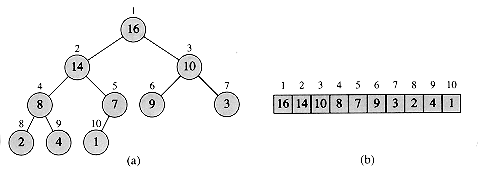
\includegraphics[width = 0.98\columnwidth]{fig/binary_tree.png}
    \caption{Max-heap be visualized with binary tree structure on the left, and implemnted with Array on the right.}
    \label{fig:max-heap-1}
\end{figure}

As we can see we can implement heap as an array due to the fact that the tree is complete. A complete binary tree is one in which each level must be fully filled before starting to fill the next level. Array-based heap is more space efficient compared with tree based due to the non-existence of the child pointers for each node. To make the math easy, we iterate node in the tree starting from root in the order of level by level and from left to right with beginning index as 1 (shown in Fig.~\ref{fig:max-heap-1}).  According to such assigning rule, the node in the tree is mapped and saved in the array by the assigned index (shown in Fig.~\ref{fig:max-heap-1}). In heap, we can traverse the imaginary binary tree in two directions:  \textbf{root-to-leaf} and  \textbf{leaf-to-root}. Given a parent node with p as index, the left child of can be found in position $2p$ in the array. Similarly, the right child of the parent is at position $2p + 1$ in the list. To find the parent of any node in the tree,  we can simply use $\lfloor p/2\rfloor$.  In Python3, use integer division $n//2$. \textit{Note: we can start index with 0 as used in \textbf{heapq} library introduced later in this section. Given a node $x$, the left and right child will be $2*x+1$, $2*x+2$, and the parent node will have index $(x-1)//2$.}

The common application of heap data structure include:
\begin{itemize}
    \item Implementing a priority-queue data structure which will be detailed in the next section so that insertion and deletion can be implemented in $O(\log n)$; Priority Queue is an important component in algorithms like Kruskal's for minimum spanning tree (MST) problem and Dijkstra's for single-source shortest paths (SSSP) problem. 
    \item Implementing heapsort algorithm,
\end{itemize}

Normally, there is usually no notion of 'search' in heap, but only insertion and deletion, which can be done by traversing a $O(\log n)$ leaf-to-root or root-to-leaf path. 
%%%%%%%%%%%%%%%%%%Basic Implementation%%%%%%%%%%%%%%%%%%%%%%%%
\subsection{Basic Implementation}
The basic methods of a heap class should include: \textbf{pop}, \textbf{push}, and \textbf{heapify}. \textbf{push} an item into the heap and \textbf{pop} the root item at the heap out, and still maintain the heap property.  And \textbf{heapify} denotes the operation needed for an given array, to convert it to a heap directly and efficiently. 

Let's implement a heap class using list. Because the first element of the heap is actually empty, we define our class as follows:
\begin{lstlisting}[language=Python]
class Heap:
    def __init__(self):
        self.heap = [None]
        self.size = 0
    def __str__(self):
        out = ''
        for i in range(1, self.size + 1):
            out += str(self.heap[i]) + ' '
        return out
\end{lstlisting}
Assuming we already have got a heap shown in Fig.~\ref{fig:max-heap-1}, push or pop an item from the current heap requires us to do post-processing in order to maintain the heap property. Let's discuss the two cases. Change it to use max heap as example.

\paragraph{Push with Floating} When we push an item into, to maintain the complete binary tree property, the new item goes to the end of the heap(array) first. Assuming the new item a[i] is the smallest item up till now, there will be violation of the heap property through the \textbf{a[i]->root path}. To correct the potential violation, we traverse the path a[i]->root, and compare each node and its parent  to decide if a swap operation is needed. For a min-heap, if the child node is smaller than the parent, that is a violation, and we swap these two nodes to let a[i] \textbf{float up} to make sure the subtree of a[i].parent obey the min-heap property.  For example, in the min-heap.  The time complexity is the same as the height of the complete tree, which is $O(\log n)$.
\begin{lstlisting}[language=Python]
    def _float(self, index): # enforce min-heap, leaf-to-root
      while index // 2: # while parent exist
          p_index = index // 2
          print('p', p_index, index)
          if self.heap[index] < self.heap[p_index]: # a violation
              # swap
              self.heap[index], self.heap[p_index] = self.heap[p_index], self.heap[index]
          else:
            break
          index = p_index # move up the node
    def insert(self, val):
        self.heap.append(val)
        self.size += 1
        self._float(index = self.size)
\end{lstlisting}

\paragraph{Pop with Sinking} When we pop out the item at root node,  or delete any item a[i], an empty spot appears at that position. To maintain the complete binary tree, we first  simply use the last item to fill in this spot. However, in a min-heap, the last item will mostly not be the smallest item among the subtree rooted at a[i]. The smallest item will appear anywhere in the subtree. We simply do a search starts from node a[i] and compare its value with left and right child. The left and right subtree obey the min-heap property already, therefore the smallest item is among a[i], left, right. If the node is larger than its smaller child node, we swap the parent with the smaller child, and move our pointer to the smaller child node and repeat the above process until the current node is the smallest among these three nodes.   This process is called like sinking down a[i] along the \textbf{path a[i]->leaf}. Same as the insert in the case of complexity, $O(\log n)$. 
\begin{lstlisting}[language=Python]
    def _sink(self, index): # enforce min-heap, root-to-leaf
        while 2 * index <= self.size:
            li = 2 * index
            ri = li + 1
            mi = index
            if self.heap[li] < self.heap[mi]:
              mi = li
            if ri <= self.size and self.heap[ri] < self.heap[mi]:
              mi = ri
            if mi != index:
                # swap index with mi
                self.heap[index], self.heap[mi] = self.heap[mi], self.heap[index]
            else:
              break
            index = mi
    def pop(self):
        val = self.heap[1]
        self.heap[1] = self. heap.pop()
        self.size -= 1
        self._sink(index = 1)
        return val
\end{lstlisting}
Now, let us run an example:
\begin{lstlisting}[language=Python]
h = Heap()
lst = [21, 1, 45, 78, 3, 5]
for v in lst:
    h.insert(v)
print('heapify with insertion: ', h)
h.pop()
print('after pop(): ', h)
\end{lstlisting}
The output is listed as:
\begin{lstlisting}
heapify with insertion: 1 3 5 78 21 45 
after pop(): 3 21 5 78 45 
\end{lstlisting}

\paragraph{Heapify with Bottom-up Sinking}  Heapify is a procedure that convert a list to a heap data structure.  We have learned the insert procedure. To heapify a list, we can do it through a series of insert iterating through the items in the list and we get an upper-bound complexity of $O(n\log n)$. However, a more efficient way to do it is is to treat the given list as a tree and to heapify directly on the list. %There are two possibly two ways to do this: (1) through sinking and (2) through floating.  
To satisfy the heap property, we need to first start from the smallest subtree. For leaf nodes, they have no children which satisfies the heap property naturally. Therefore we can jumpy to the last parent node, which will be at position a[n//2]. We apply the sinking process as used in \textbf{pop} so that this subtree rooted at current node obeys the heap property. And we   iterate through all the parents nodes that is a[1...n//2] in reversed order, we can guarentee that final complete binary tree still obeys the heap property. This follows a divide-and-conquer (DP) fashion. Instead of heaipfy A[1...n], we first, heaipfy A[n], A[n-1...n], A[n-2...n], ..., A[1...n].  The process is shown in Fig.~\ref{fig:heapify}. With this process, it can give us a tighter upper bound and close to $O(n)$. 
\begin{figure}[h!]
    \centering
    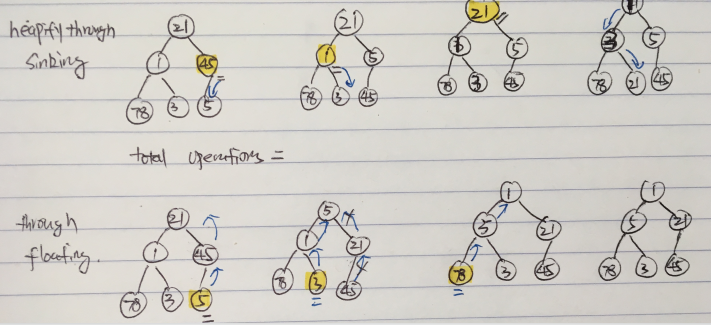
\includegraphics[width = 0.98\columnwidth]{fig/heapify.png}
    \caption{Heapify for a given list.}
    \label{fig:heapify}
\end{figure}
\begin{lstlisting}[language=Python]
  def heapify_sink(self, lst):
      self.heap = [None] + lst
      self.size = len(lst)
      for i in range(self.size//2, 0, -1):
        self._sink(i)
\end{lstlisting}

Now, run the following code:
\begin{lstlisting}[language=Python]
h = Heap()
h.heapify(lst)
print('heapify with heapify:', h)
\end{lstlisting}
Out put is:
\begin{lstlisting}
heapify with heapify: 1 5 21 78 3 45 
\end{lstlisting}
\begin{bclogo}[couleur = blue!30, arrondi=0.1,logo=\bccrayon,ombre=true]{Which way is more efficient building a heap from a list?} Using insertion or heapify? What is the efficiency of each method? The experimental result can be seen in the code.
\end{bclogo}
When we are solving a problem, unless specifically required for implementation, we can always use an existent Python module/package. Here, we introduce one Python module: heapq that implements heap data structure for us. 
% \begin{enumerate}
% \item MAX-HEAPIFY, runs in $O(lgn)$, is the key to maintaining the max-heap property
% \item BUILD-MAX-HEAP, runs in linear time, produces a maxheap from an unordered input array
% \item MAX-HEAP-INSERT, HEAP-EXTRACT-MAX, HEAP-INCREASE-KEY, and HEAP-MAXIMUM, runs in $O(lgn)$ time, allow the heap data structure to implement a priority queue
% \end{enumerate}
%%%%%%%%%%%%%%%%%%Python Built-in Module: heapq%%%%%%%%%%%%%%%%%%%%%%%%
\subsection{Python Built-in Library: heapq}
\textbf{heapq}: heapq is a built-in library in Python that implements relevant functions to carry out various operations on heap data structure. These functions are listed and described in Table~\ref{tab:functions_in_heapq}. \textit{To note that heapq is not a data type like queue.Queue() or collections.deque(), it is a library (or class) that can do operations like it is on a heap.} %, which can be used to maintain a priority queue. Operations include heappush, heappop, and nsmallest. heapq in python to maintain a priority queue with $O(logn)$.
\begin{table}[h]
\begin{small}
\centering
\noindent\captionof{table}{ Methods of \textbf{heapq}}
 \noindent \begin{tabular}{|p{0.25\columnwidth}|p{0.75\columnwidth}| }
  \hline
Method & Description   \\ \hline
heappush(h, x)  &  Push the value item onto the heap, maintaining the heap invariant.  \\\hline
heappop(h)  &Pop and return the \textit{smallest} item from the heap, maintaining the heap invariant. If the heap is empty, IndexError is raised.\\ \hline
heappushpop(h, x)  &Push item on the heap, then pop and return the smallest item from the heap. The combined action runs more efficiently than heappush() followed by a separate call to heappop().\\ \hline
heapify(x) & Transform list x into a heap, in-place, in linear time.\\ \hline
heapreplace(h, x) & Pop and return the smallest item from the heap, and also push the new item. The heap size doesn’t change. If the heap is empty, IndexError is raised. This is more efficient than heappop() followed by heappush(), and can be more appropriate when using a fixed-size heap.\\ \hline
nlargest(k, iterable, key = fun) & This function is used to return the k largest elements from the iterable specified and satisfying the key if mentioned. \\ \hline
nsmallest(k, iterable, key = fun) & This function is used to return the k smallest elements from the iterable specified and satisfying the key if mentioned. \\ \hline
\end{tabular}
  \label{tab:functions_in_heapq}
  \end{small}
\end{table} 
heapq has some other functions like merge(), nlargest(), nsmallest() that we can use. Check out \url{https://docs.python.org/3.0/library/heapq.html} for more detials. 

\paragraph{Min-Heap} Now, let us try to heapify the same examplary list as used in the last section, [21, 1, 45, 78, 3, 5], we use need to call the function heapify(). The time complexity of heapify is $O(n)$
\begin{lstlisting}[language = Python]
'''implementing with heapq'''
from heapq import heappush, heappop, heapify
h = [21, 1, 45, 78, 3, 5]
heapify(h) # inplace
print('heapify with heapq: ', h)
\end{lstlisting}
The print out is:
\begin{lstlisting}
heapify with heapq:  [1, 3, 5, 78, 21, 45]
\end{lstlisting}

 Here we demonstrate how to use function nlargest() and nsmallest() if getting the first n largest or smallest is what we need, we do not need to heapify() the list as we needed in the heap and pop out the smallest. The step of heapify is built in these two functions.
\begin{lstlisting}[language=Python]
''' use heapq to get nlargest and nsmallest'''
li1 = [21, 1, 45, 78, 3, 5]
# using nlargest to print 3 largest numbers
print("The 3 largest numbers in list are : ", end="")
print(heapq.nlargest(3, li1))

# using nsmallest to print 3 smallest numbers
print("The 3 smallest numbers in list are : ", end="")
print(heapq.nsmallest(3, li1))
\end{lstlisting}
The print out is:
\begin{lstlisting}
The 3 largest numbers in list are : [78, 45, 21]
The 3 smallest numbers in list are : [1, 3, 5]
\end{lstlisting}


\paragraph{Max-Heap} As we can see the default heap implemented in the heapq library is forcing the heap property of the min-heap. What if we want a max-heap instead? In heapq library, it does offer us function, but it is intentionally hided from users. It can be accessed like: heapq.\_[function]\_max(). Now, let us implement a max-heap instead. 
\begin{lstlisting}[language = Python]
# implement a max-heap
h = [21, 1, 45, 78, 3, 5]
heapq._heapify_max(h) # inplace
print('heapify max-heap with heapq: ', h)
\end{lstlisting}
The print out is:
\begin{lstlisting}
heapify max-heap with heapq:  [78, 21, 45, 1, 3, 5]
\end{lstlisting}

Also, in practise, a simple hack for the max-heap is to save data as negative. Also, in the priority queue.
% What is we want a max-heap which returns the largest number instead of the smallest each time? 
% \subsubsection{Max-heap and Min-heap}
% We can write our own MinHeap and MaxHeap class wrapper as follows so that it can be easier to use:
% \begin{lstlisting}[language = Python]
% class MaxHeapObj(object):
%     def __init__(self,val): self.val = val
%     def __lt__(self,other): return self.val > other.val
%     def __eq__(self,other): return self.val == other.val
%     def __str__(self): return str(self.val)
    
% class MinHeap(object):
%     def __init__(self): self.h = []
%     def heappush(self,x): heapq.heappush(self.h,x)
%     def heappop(self): return heapq.heappop(self.h)
%     def __getitem__(self,i): return self.h[i]
%     def __len__(self): return len(self.h)

% class MaxHeap(MinHeap):
%     def heappush(self,x): heapq.heappush(self.h,MaxHeapObj(x))
%     def heappop(self): return heapq.heappop(self.h).val
%     def __getitem__(self,i): return self.h[i].val
% \end{lstlisting}
\paragraph{More Private Functions}
\begin{table}[h]
\begin{small}
\centering
\noindent\captionof{table}{ Private Methods of \textbf{heapq}}
 \noindent \begin{tabular}{|p{0.25\columnwidth}|p{0.75\columnwidth}| }
  \hline
Method & Description   \\ \hline
heappush(h, x)  &  Push the value item onto the heap, maintaining the heap invariant.  \\\hline
heappop(h)  &Pop and return the \textit{smallest} item from the heap, maintaining the heap invariant. If the heap is empty, IndexError is raised.\\ \hline
heappushpop(h, x)  &Push item on the heap, then pop and return the smallest item from the heap. The combined action runs more efficiently than heappush() followed by a separate call to heappop().\\ \hline
heapify(x) & Transform list x into a heap, in-place, in linear time.\\ \hline
heapreplace(h, x) & Pop and return the smallest item from the heap, and also push the new item. The heap size doesn’t change. If the heap is empty, IndexError is raised. This is more efficient than heappop() followed by heappush(), and can be more appropriate when using a fixed-size heap.\\ \hline
nlargest(k, iterable, key = fun) & This function is used to return the k largest elements from the iterable specified and satisfying the key if mentioned. \\ \hline
nsmallest(k, iterable, key = fun) & This function is used to return the k smallest elements from the iterable specified and satisfying the key if mentioned. \\ \hline
\end{tabular}
  \label{tab:functions_in_heapq}
  \end{small}
\end{table} 

\paragraph{With Tuple/List or Customized Object as Elements}
Any object that supports comparison (\texttt{\_cmp\_()}) can be used in heap with \texttt{heapq}. When we want our item includes information as (priority, task), we can either put it in tuple or list. In the heap, we can change the value of any item just as in the list. However, the problem occurs after the change that the list will violate the heap priority. What we can do is use function such as \texttt{\_siftdown(heap, 0, len(heap)-1)} (used to implement heappush, and called with decreased priority ) and \texttt{\_siftup(heap, 0)} (used to implement heappop, and called with increased priority). 
\begin{lstlisting}[language=Python]
import heapq

heap = [[3, 'a'], [10, 'b'], [5,'c']]
heapq.heapify(heap)
print(heap)

heap[0] = [6, 'a']
print(heap)
heapq._siftup(heap, 0) #simlar to remove heap[0], put this item at the end
print(heap)
\end{lstlisting}

%%%%%%%%%%%%%%%%%%%%priority Queue%%%%%%%%%%%%%%%%%%%
\section{Priority Queue}
\label{sec_priority_queue}
A priority queue is an abstract data type(ADT) and an extension of queue with properties: (1) additionally each item has a priority associated with it. (2) In a priority queue, an item with high priority is served (dequeued) before an item with low priority. (3) If two items have the same priority, they are served according to their order in the queue. 

Heap is generally preferred for priority queue implementation because of its better performance compared with arrays or linked list. Also, in Python queue module, we have \texttt{PriorityQueue()} class that provided us the implementation. Beside, we can can implement priority queue with  \texttt{heapq} library too. These contents will be covered in the next two subsection. 

Applications of Priority Queue:
\begin{enumerate}
    \item CPU Scheduling
    \item Graph algorithms like Dijkstra’s shortest path algorithm, Prim’s Minimum Spanning Tree, etc
    \item All queue applications where priority is involved. 
\end{enumerate}

\subsubsection{Implement with \texttt{heapq}  Library} The core function is the ones used to implement the heap: \texttt{heapify()}, \texttt{push()}, and \texttt{pop()}. The official document:\url{https://docs.python.org/2/library/heapq.html} gave the exact implementation. However, we are still going to summarize and organize this information in our book. In order to implement priority queue, our binary heap needs to have the following features:
\begin{enumerate}
    \item Sort stability: when we get two tasks with equal priorities, we return them in the order as of they were originally added. A potential solution is to modify the original 2-element list (priority, task) into a 3-element list as (priority, count, task). The entry \texttt{count} serves as a tie-breaker so that two tasks with the same priority are returned in the order they were added. And also, since no two entry counts are the same the tuple comparison will never attemp to directly compare two tasks.
    \item Find a task in the heap, and either remove it or update its priority. Situations like the priority of a task changes or if a pending task needs to be removed. We understand how inconvenient it can be to find the non-root item and update its value. Normally, finding the item is a linear search which takes $O(n)$ and update its value using either \texttt{\_siftdown()} or \texttt{\_siftup()} can be $O(\log n)$. The solution is: (1) do not remove the task other than the \texttt{pop} operation, but mark it as REMOVED instead; (2) to define a dictionary that use \texttt{task} as key and the 3-element list as value. We name it \texttt{entry\_finder}. When the entry is a list, in the heap that encompass these items will only get pointers. Therefore, we can execute the find/mark as removed operation using task as key and do it in the \texttt{entry\_finder} instead.
\end{enumerate}
Python code:
\begin{lstlisting}[language=Python]
from heapq import heappush, heappop, heapify
from typing import List
import itertools
class PriorityQueue:
  def __init__(self, items:List[List]=[]):
      self.pq = []                         # list of entries arranged in a heap
      self.entry_finder = {}               # mapping of tasks to entries
      self.REMOVED = '<removed-task>'      # placeholder for a removed task
      self.counter = itertools.count()     # unique sequence count
      # add count to items
      for p, t in items:
        item = [p, next(self.counter), t]
        self.entry_finder[t] = item
        self.pq.append(item)
      heapify(self.pq)
        
  def add_task(self, task, priority=0):
      'Add a new task or update the priority of an existing task'
      if task in self.entry_finder:
          self.remove_task(task)
      count = next(self.counter)
      entry = [priority, count, task]
      self.entry_finder[task] = entry
      heappush(self.pq, entry)
      
  def remove_task(self, task):
      'Mark an existing task as REMOVED.  Raise KeyError if not found.'
      entry = self.entry_finder.pop(task)
      entry[-1] = self.REMOVED

  def pop_task(self):
      'Remove and return the lowest priority task. Raise KeyError if empty.'
      while self.pq:
          priority, count, task = heappop(self.pq)
          if task is not self.REMOVED:
              del self.entry_finder[task]
              return task
      raise KeyError('pop from an empty priority queue')
\end{lstlisting}
Let's run an example with our customized \texttt{PriorityQueue} class:
\begin{lstlisting}[language=Python]
pq = PriorityQueue(items=[[6, 'task 6'], [5, 'task5'], [19, 'task19']])
print(pq.pq)
pq.add_task('task 10', 10)
print(pq.pq)
pq.remove_task('task5')
print(pq.pq)
pq.pop_task()
\end{lstlisting}
With output as:
\begin{lstlisting}[numbers=none]
[[5, 1, 'task5'], [6, 0, 'task 6'], [19, 2, 'task19']]
[[5, 1, 'task5'], [6, 0, 'task 6'], [19, 2, 'task19'], [10, 3, 'task 10']]
[[5, 1, '<removed-task>'], [6, 0, 'task 6'], [19, 2, 'task19'], [10, 3, 'task 10']]
'task 6'
\end{lstlisting}

\subsubsection{Implement with \texttt{PriorityQueue} class} Class \texttt{PriorityQueue()} is the same as \texttt{Queue()}, \texttt{LifoQueue()}, they have same member functions as shown in Table~\ref{tab:methods_of_queue}. Therefore, we skip the semantic introduction. \texttt{PriorityQueue()} normally thinks that the smaller the value is the higher the priority is. We use a similar example as above to demonstrate its function. 
\begin{lstlisting}[language=Python]
import queue
pq = queue.PriorityQueue()
items=[[6, 'task 6'], [5, 'task5'], [19, 'task19']]
for item in items:
  pq.put(item)

print(pq.queue)
next_job = pq.get()
print('processing job:', next_job)
print(pq.queue)
\end{lstlisting}
The output is:
\begin{lstlisting}
[[5, 'task5'], [6, 'task 6'], [19, 'task19']]
processing job: [5, 'task5']
[[6, 'task 6'], [19, 'task19']]
\end{lstlisting}
If we want to give the number with larger value as higher priority, a simple hack is to pass by negative value. Another more professional way is to pass by a customized object and rewrite the comparison operator: < and == in the class with \_\_lt\_\_() and \_\_eq\_\_(). In the following code, we show how to use higher value as higher priority. 
\begin{lstlisting}[language = Python]
class Job(object):
    def __init__(self, priority, description):
        self.priority = priority
        self.description = description
        print('New job:', description)
        return
    # def __cmp__(self, other):
    #     return cmp(self.priority, other.priority)
    '''customize the comparison operators '''
    def __lt__(self, other): # <
        try:
            return self.priority > other.priority
        except AttributeError:
            return NotImplemented
    def __eq__(self, other): # ==
        try:
            return self.priority == other.priority
        except AttributeError:
            return NotImplemented

q = Queue.PriorityQueue()

q.put( Job(3, 'Mid-level job') )
q.put( Job(10, 'Low-level job') )
q.put( Job(1, 'Important job') )

while not q.empty():
    next_job = q.get()
    print('Processing job:', next_job.priority)
\end{lstlisting}
The print out is:
\begin{lstlisting}
Processing job: 10
Processing job: 3
Processing job: 1
\end{lstlisting}
If we want the priority queue to be able to update the priority of a task, we can apply similar wrapper in the \texttt{heapq} section. 
\begin{bclogo}[couleur = blue!30, arrondi=0.1,logo=\bccrayon,ombre=true]{In single thread programming, is \textbf{heapq} or \textbf{PriorityQueue} more efficient?} In fact, the PriorityQueue implementation uses heapq under the hood to do all prioritisation work, with the base Queue class providing the locking to make it thread-safe. While heapq module offers no locking, and operates on standard list objects. This makes the heapq module faster; there is no locking overhead. In addition, you are free to use the various heapq functions in different, noval ways, while the PriorityQueue only offers the straight-up queueing functionality. 
\end{bclogo}
Let us take these knowledge into practice with a LeetCode Problem:
347. Top K Frequent Elements (medium). Given a non-empty array of integers, return the k most frequent elements.
\begin{lstlisting}[numbers=none]
Example 1:

Input: nums = [1,1,1,2,2,3], k = 2
Output: [1,2]

Example 2:

Input: nums = [1], k = 1
Output: [1]
\end{lstlisting}

Analysis: to solve this problem, we need to first using a hashmap to get information as: item and its freqency. Then, we need to obtain the top frequent elements. The second step can be down with sorting, or using heap we learned.

\textbf{Solution 1: Use Counter().} Counter() has a function most\_common(k) that will return the top k most frequent items. However, its complexity will be $O(n \log n)$. 
\begin{lstlisting}[language=Python]
from collections import Counter
def topKFrequent(self, nums, k):
    return [x for x, _ in Counter(nums).most_common(k)]
\end{lstlisting}

\textbf{Solution 2: Use dict and heapq.nlargest()}. The complexity should be better than $O(n \log n)$. 
\begin{lstlisting}[language=Python]
from collections import Counter
import heapq
def topKFrequent(self, nums, k):
    count = collections.Counter(nums)   
    return heapq.nlargest(k, count.keys(), key=count.get) 
\end{lstlisting}

We can also use PriorityQueue(). 
\begin{lstlisting}[language=Python]
from queue import PriorityQueue
class Solution:
def topKFrequent(self, nums, k):
    h = PriorityQueue()
    
    # build a hashmap (element, frequency)
    temp = {}
    for n in nums:
        if n not in temp:
            temp[n] = 1
        else:
            temp[n] += 1
    # put them as (-frequency, element) in the queue or heap
    for key, item in temp.items():
        h.put((-item, key))
    
    # get the top k frequent ones
    ans = [None]*k
    for i in range(k):
        _, ans[i] = h.get()
    return ans
\end{lstlisting}

\section{Bonus}
\label{heap_sec_bonus}
\paragraph{Fibonacci heap} With fibonacc heap, insert() and getHighestPriority() can be implemented in O(1) amortized time and deleteHighestPriority() can be implemented in O(Logn) amortized time.
%%%%%%%%%%%%%%%%%%%%%%%LeetCode problems%%%%%%%%%%%%%%%%%%%%%%%%%%%%%%%%%%%%
\section{Exercises}

\textbf{selection with key word: kth. These problems can be solved by sorting, using heap, or use quickselect}
\begin{enumerate}
\item 703. Kth Largest Element in a Stream (easy)
    \item 215. Kth Largest Element in an Array (medium)
    \item 	347. Top K Frequent Elements (medium)
    \item 373. Find K Pairs with Smallest Sums (Medium	
	\item 378. Kth Smallest Element in a Sorted Matrix (medium)
\end{enumerate}
\textbf{priority queue or quicksort, quickselect}
\begin{enumerate}
    \item 23. Merge k Sorted Lists (hard)
    \item 253. Meeting Rooms II (medium)
    \item 621. Task Scheduler (medium)
\end{enumerate}
\end{document}